\documentclass{standalone}

\usepackage[british]{babel}
\usepackage{graphicx}
%\usepackage{epstopdf,epsfig}
\usepackage{newtxtext}
\usepackage{newtxmath}
\usepackage{natbib}
\usepackage{hyperref}

\usepackage[usenames,x11names]{xcolor}
\usepackage{tikz}
\usetikzlibrary{shapes.geometric, arrows, intersections, through}
\usetikzlibrary{arrows.meta}
\usetikzlibrary{calc}
\tikzset{math3d/.style={z={(-0.65cm,-0.30cm)},y={(0cm,1cm)},x={(0.9cm,-0.15cm)}}}
\usetikzlibrary{shapes.geometric, arrows, intersections, through}
\usetikzlibrary{decorations.text, decorations.shapes, backgrounds}
\usetikzlibrary{arrows.meta}


\begin{document}


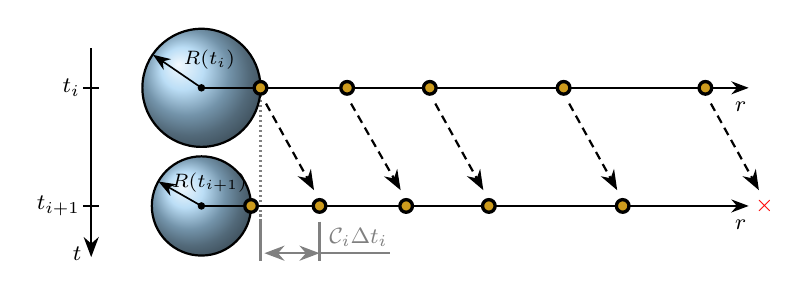
\begin{tikzpicture}[scale=1]
        \draw[thick, gray, densely dotted] (0.65,-0.2) -- (0.65,1.45);
        \shadedraw[thick,ball color = SkyBlue2!70] (-0.1,1.5) circle (0.75);
        \draw[semithick,-{Stealth[scale=1.1]}] (-0.1,1.5) -- (-0.715,1.92);
        \draw (0,1.86) node{\scriptsize $R(t_{i})$};
        \draw[black,fill=black] (-0.1,1.5) circle (0.04);
        \draw[semithick,-{Stealth[scale=1.1]}] (-0.1,1.5) -- (6.85,1.5);
        \draw (6.75,1.45) node[below]{\footnotesize $r$};
        \draw[black,very thick,fill=Goldenrod3] (0.65,1.5) circle (0.08);
        \draw[black,very thick,fill=Goldenrod3] (1.75,1.5) circle (0.08);
        \draw[black,very thick,fill=Goldenrod3] (2.8,1.5) circle (0.08);
        \draw[black,very thick,fill=Goldenrod3] (4.5,1.5) circle (0.08);
        \draw[black,very thick,fill=Goldenrod3] (6.3,1.5) circle (0.08);
        \shadedraw[thick,ball color = SkyBlue2!70] (-0.1,0) circle (0.63);
        \draw[semithick,-{Stealth[scale=1.1]}] (-0.1,0) -- (-0.645,0.31);
        \draw (-0.0,0.3) node{\scriptsize $R(t_{i+1})$};
        \draw[black,fill=black] (-0.1,0) circle (0.04);
        \draw[semithick,-{Stealth[scale=1.1]}] (-0.1,0) -- (6.85,0);
        \draw (6.75,-0.05) node[below]{\footnotesize $r$};
        \draw[black,very thick,fill=Goldenrod3] (0.53,0) circle (0.08);
        \draw[black,very thick,fill=Goldenrod3] (1.4,0) circle (0.08);
        \draw[black,very thick,fill=Goldenrod3] (2.5,0) circle (0.08);
        \draw[black,very thick,fill=Goldenrod3] (3.55,0) circle (0.08);
        \draw[black,very thick,fill=Goldenrod3] (5.25,0) circle (0.08);
        \draw (7.05,0) node{\footnotesize {\color{red} $\boldsymbol{\times}$}};
        \draw[densely dashed,thick,-{Stealth[scale=1.1]}] (0.72,1.3) -- (1.33,0.2);
        \draw[densely dashed,thick,-{Stealth[scale=1.1]}] (1.8,1.3) -- (2.43,0.2);
        \draw[densely dashed,thick,-{Stealth[scale=1.1]}] (2.87,1.3) -- (3.48,0.2);
        \draw[densely dashed,thick,-{Stealth[scale=1.1]}] (4.57,1.3) -- (5.18,0.2);
        \draw[densely dashed,thick,-{Stealth[scale=1.1]}] (6.37,1.3) -- (6.98,0.2);
        \draw[thick,-{Stealth[scale=1.1]}] (-1.5,2) -- (-1.5,-0.65);
        \draw[thick] (-1.6,1.5) -- (-1.4,1.5);
        \draw[thick] (-1.6,0) -- (-1.4,0);
        \draw (-1.52,1.5) node[left]{\footnotesize $t_{i}$};
        \draw (-1.52,0) node[left]{\footnotesize $t_{i+1}$~};
%                \draw (-1.52,0) node[left]{\footnotesize $t_{i}=t_{i-1} + \Delta t_{i-1}$~};
        \draw (-1.5,-0.6) node[left]{\footnotesize $t$};
        \draw[thick, gray] (0.65,-0.2) -- (0.65,-0.7);
        \draw[thick, gray] (1.4,-0.2) -- (1.4,-0.7);
        \draw[thick, gray, {Stealth[scale=1.1]}-{Stealth[scale=1.1]}] (0.7,-0.6) -- (1.4,-0.6);
        \draw[thick, gray] (1.4,-0.6) -- (2.3,-0.6);
        \draw (1.4,-0.4) node[right, gray]{\footnotesize $\mathcal{C}_i \Delta t_{i}$};
    \end{tikzpicture}
    

\end{document}
